
\chapter{Introduction}

	One of the main topics in computer vision is object recognition. Despite many years of research that brought us all kinds of artificial algorithms, very basic problems remain nearly unsolvable.
	
	An example would be this simple decision task: Is there a bird in an image? Humans can answer this after seeing a picture for only very short duration although they never saw the image before. More surprisingly it also does not matter if a person knows that exact type of bird or if he had seen it before. Viewing positions and angles, photometric effects, scene settings and changing body shapes have little effect on the overall test performance.
	
	It is obvious this is the product of a long evolutionary process that lead to a high efficient object recognition system like the one in humans. So if it works this well, the naive solution is to design new algorithms the same way the human visual system works.
	
	To gain an understanding of what these new models should achieve, we are starting to look at the physiology in chapter 2. After covering the anatomy of the retina and the information transport to the brain, the complexity of the visual cortex will be addressed.
	
	Chapter 3 starts off with some background about what kind of model will be used. The basis for all of them will be the results of \citeauthor{hubel1962receptive}'s research that is shortly explained and then used to implement the HMAX model by \citeauthor{riesenhuber1999hierarchical}. \citeauthor{serre2007robust} refined this model and also discussed the biological plausibility. To emphasize the performance of the developed models this chapter concludes with a comparison to artificial state-of-the-art algorithms.
	
	As the main task of this seminar is to find a biological inspired way for self-localization, chapter 4 comes back to that and links the acquired models to that application. It is basically object recognition but with some boundary conditions and many additional work.
	
	
% todo: Title?
\chapter{Human Visual System}

	Until today the human vision is the best-known system for recognizing objects and actions in a scene is a very short time. The basis to understand how it works lies in the anatomy and physiology. Therefore all the parts that belong to the visual cortex are described here.
	
	\section{Retina}
		
		The retina is the only source for visual stimuli in mammals. This is an excellent prerequisite to study neural responses, because all input can easily be controlled.
		
		Figure \ref{retina-cross-section} shows a cross section through a human eye. Light enters through the lens that (ideally) focuses a sharp image onto the foeva. The foeva is the part of the retina with the highest density of cells and is the area with which humans most consciously see. The photons travel through all layers before getting absorbed and transfered into neuronal signals at the photo receptors.
		
		\begin{figure}[H]
			\centering
			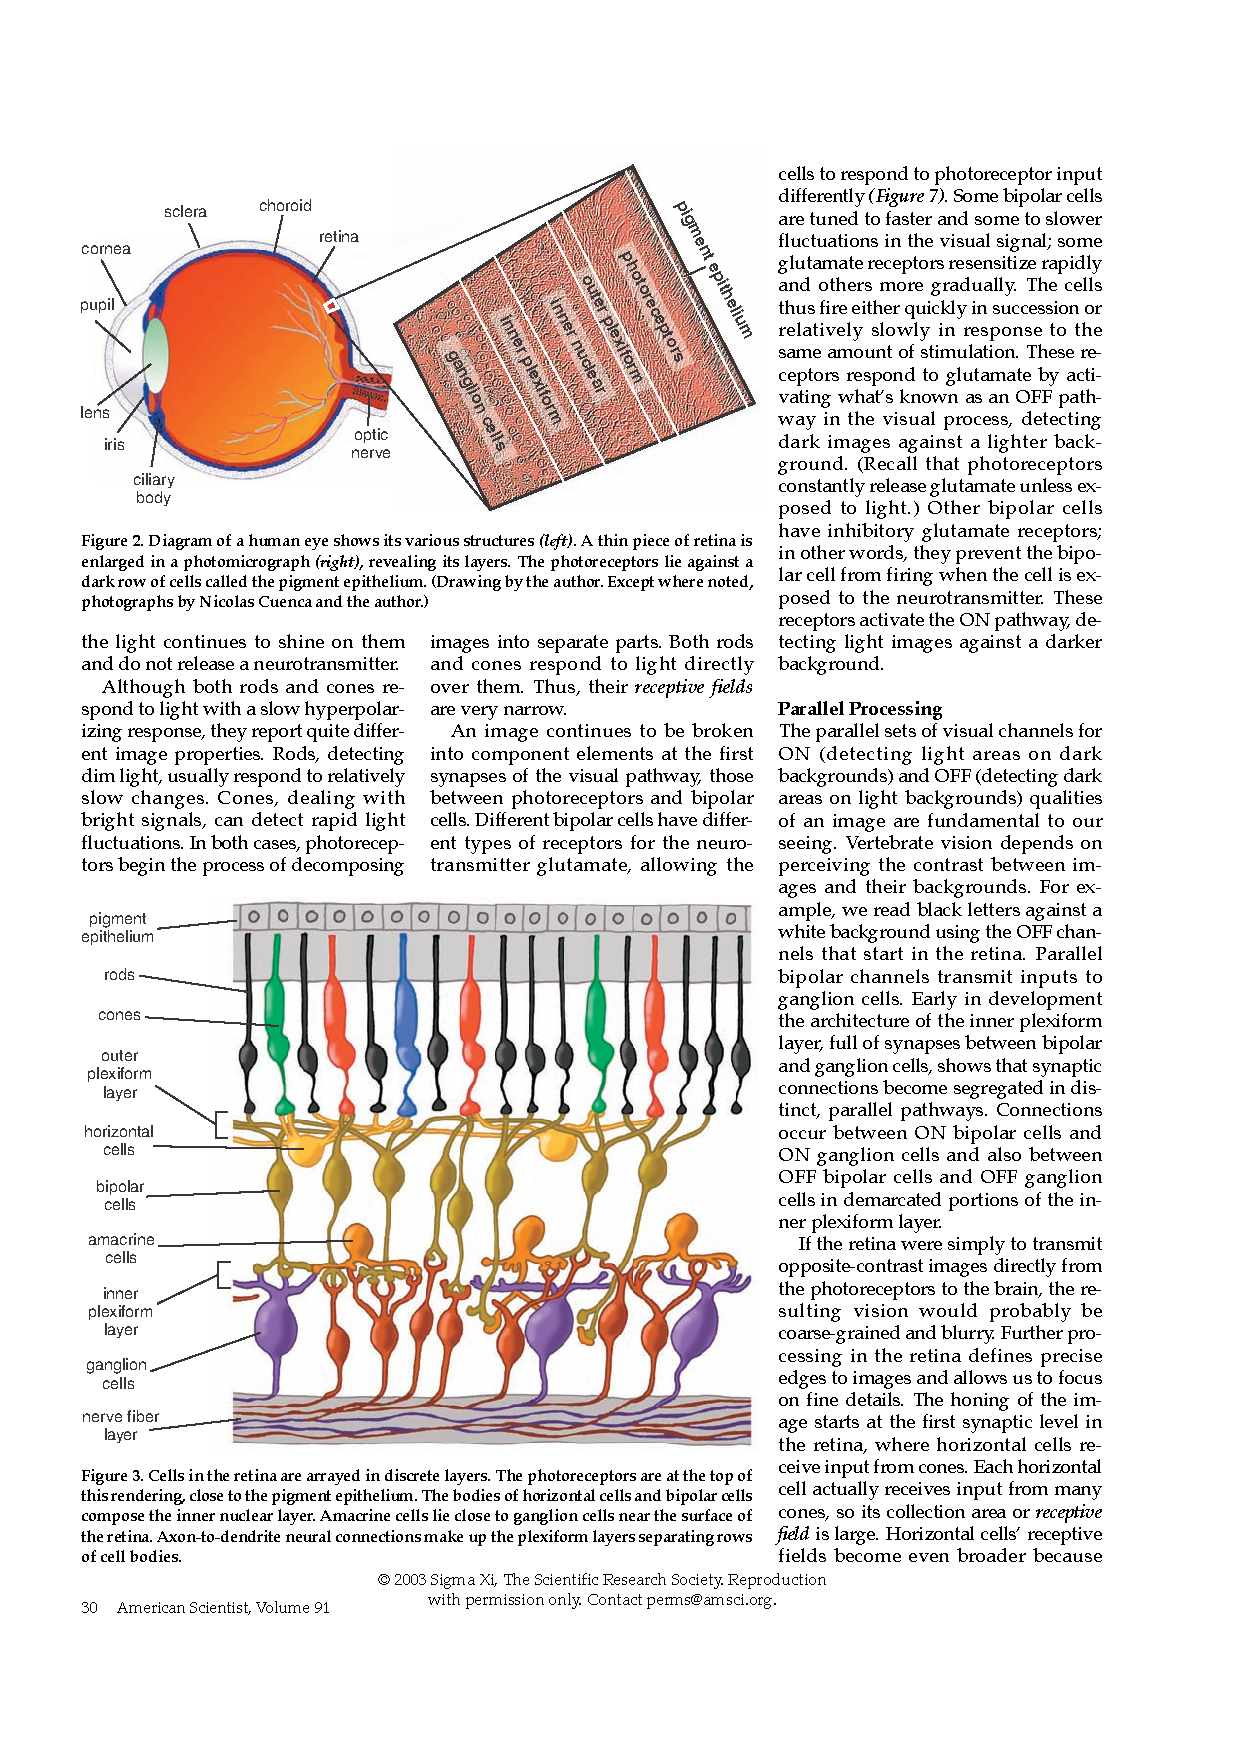
\includegraphics[width=0.8\textwidth, trim=1cm 21cm 8cm 2.5cm, clip]{images/kolb-2003-howtheretinaworks-p3.pdf}
			\caption{Cross section of the human eye \citep{kolb2003retina}}
			\label{retina-cross-section}
		\end{figure}
		
		There is already processing happening in the layers of the retina before the information goes on the optic nerve. The photo receptive cells, the rods and cones, generate an analog signal in the outer plexiform layer. This is the input of the bipolar cells that transport the signal to the inner plexiform layer. With interaction between bipolar and horizontal cells, the visual system is able to adapt to different illuminations. In the inner plexiform layer the dentrites of ganglion cells and amacrines combine the data from different bipolar cells before it get converted to action potentials and sent out of the retina.
		
		Overall the information is encoded into a string of about 1 million ganglion axons that are called the optic nerve. It transports the information to the optic chiasm.
		
		\begin{figure}[H]
			\centering
			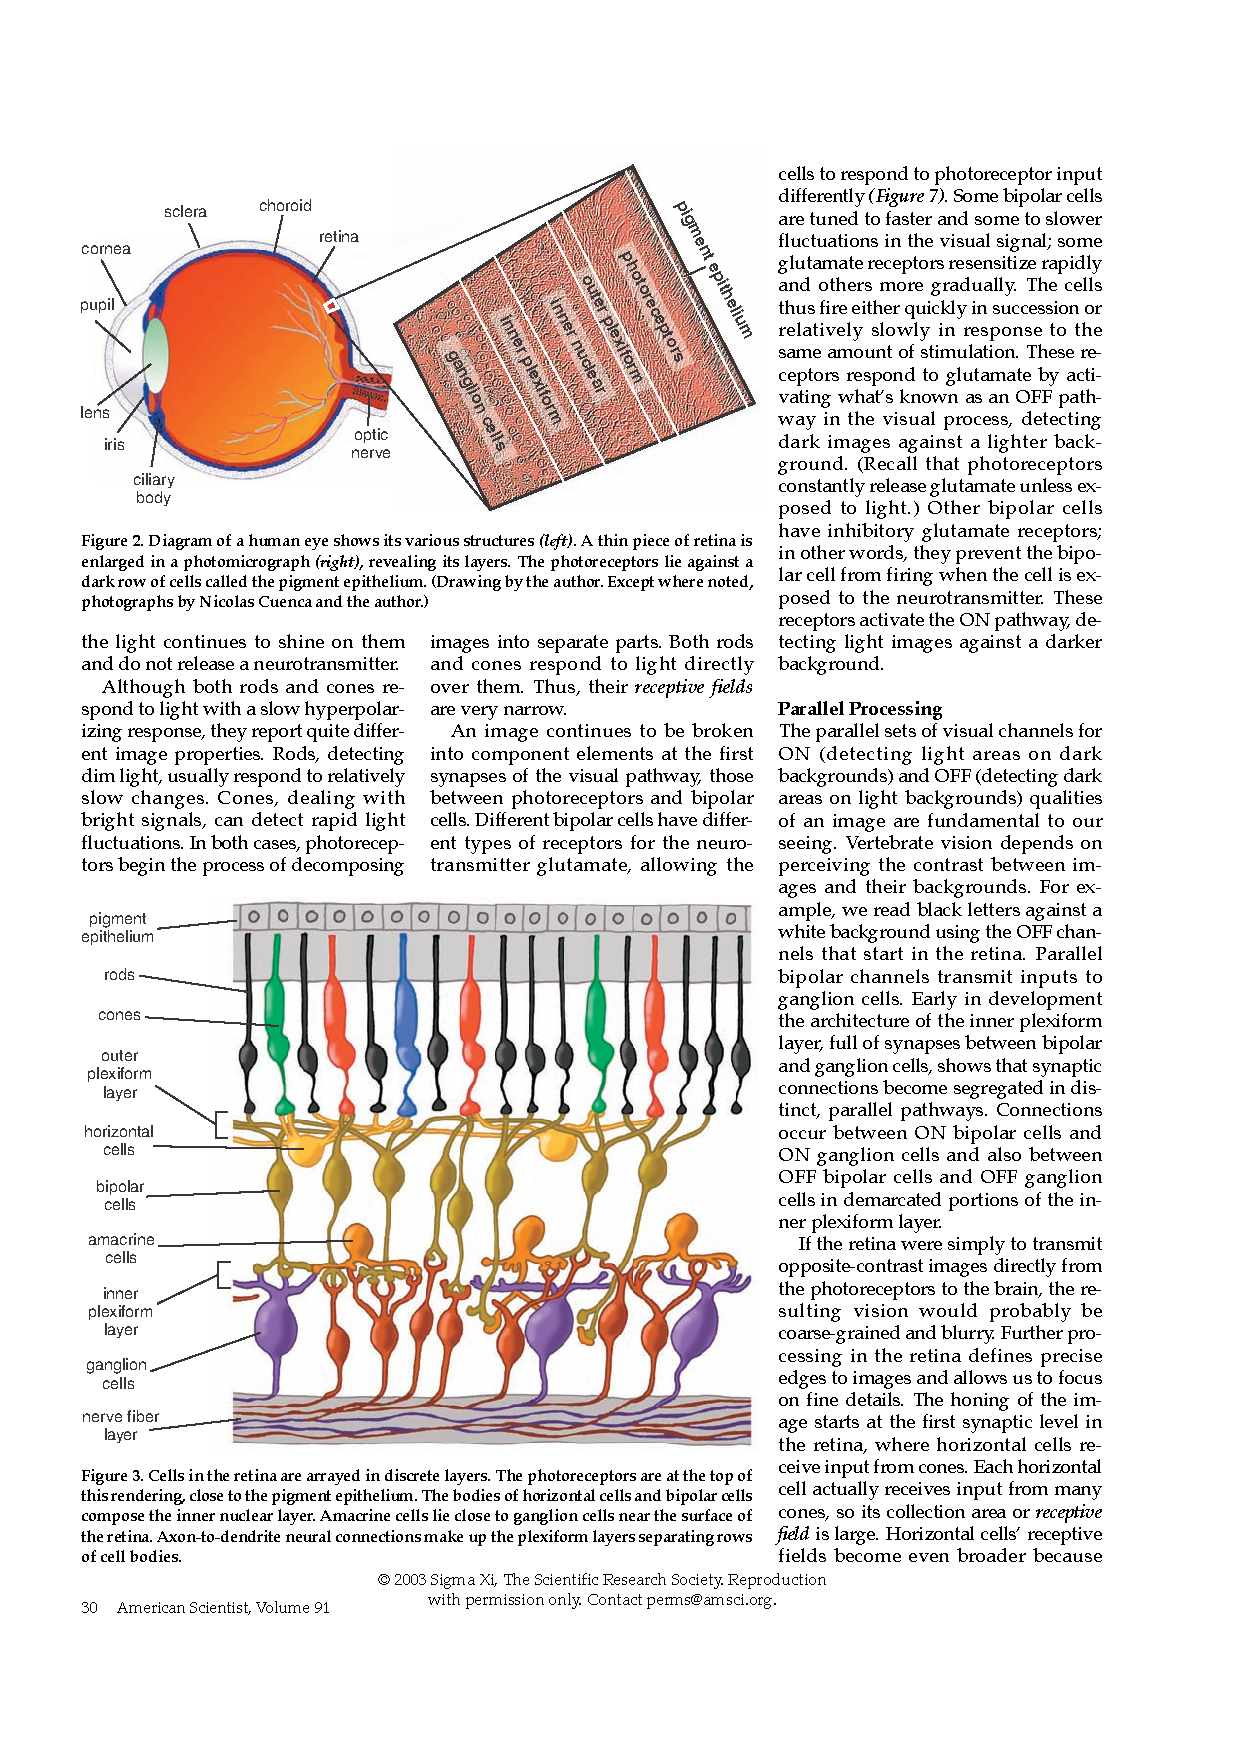
\includegraphics[width=0.8\textwidth, trim=1cm 5cm 8cm 15cm, clip]{images/kolb-2003-howtheretinaworks-p3.pdf}
			\caption{Cross section of the retina \citep{kolb2003retina}}
		\end{figure}
		
		So what is the output of the retina?
		
		%todo
		
		\begin{figure}[H]
			\centering
			\captionsetup{justification=centering,margin=0.5cm}
			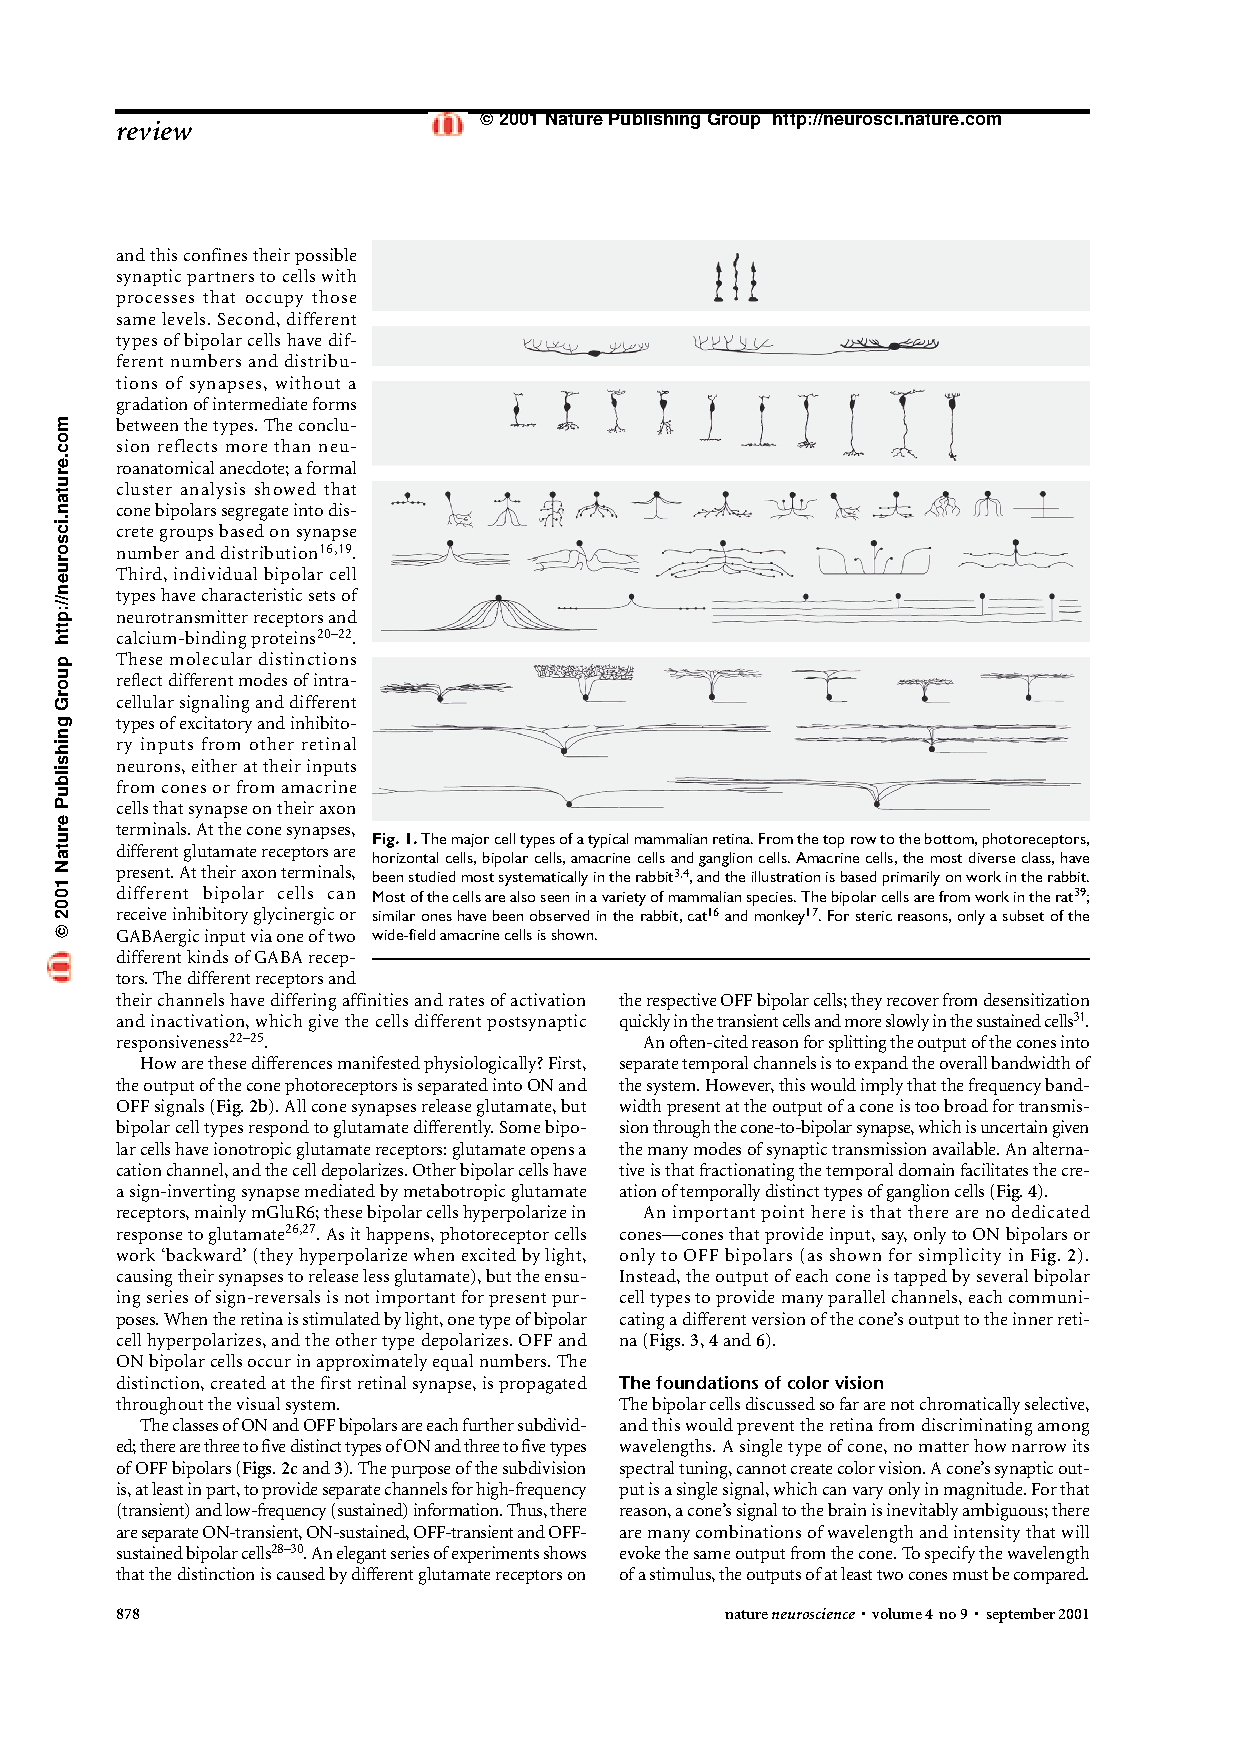
\includegraphics[width=\textwidth, trim=6.2cm 15.7cm 2cm 4cm, clip]{images/masland-2001-neuron-types.pdf}
			\caption{Different types of neuroes in the layers of the retina (from top): photo receptors, horizontal cells, bipolar cells, amacrine cells and ganglion cells \citep{masland2001fundamental}}
		\end{figure}
		
		output:
			- mainly to the LGN and from then on in the primary visual cortex
			- other low level functions: pupil control, shut lids on flash, ...
		
		output characteristics:
			- everything happens in parallel
			
		special low level function:
			- inhibit signals caused by eye or head movement (object motion sensitive cells)

	\section{Optic Chiasm and Lateral Geniculate Nucleus}
	
		In the optic chiasm the signals on the optic nerve are separated into the left and right half frame of the eye. Then the same side signals from both eyes are sent together to the lateral geniculate nucleus (LGN).

		\begin{figure}[H]
			\centering
			\captionsetup{justification=centering,margin=1cm}
			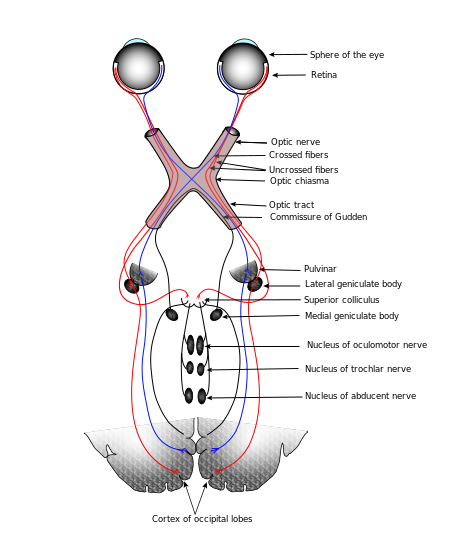
\includegraphics[width=0.7\textwidth]{images/optic-chiasm.png}
			\caption{Overview of the signal flow from the eyes (top) to the visual cortex (bottom), blue lines indicate the nasal side of retinal signals, red the temporal ones}
		\end{figure}

		The major processes that happen in the LGN have to do with combining the signals from the left and right eye. This has little effect on the ability to recognize objects simply because this also works with only one eye.
		
	
	\section{Visual Cortex}
	
		The human visual cortex is the biggest single part of the brain. This emphasizes the major role vision has for humans. In about 20 distinct areas the incoming signals from the retina are processed in a mostly hierarchically manner.
		
		Many different regions were identified to perform distinct tasks. Figure \ref{cortex-map} is an example of a map of the connections between these areas. Most of them are bidirectional.

		\begin{figure}[H]
			\centering
			\captionsetup{justification=centering,margin=0.5cm}
			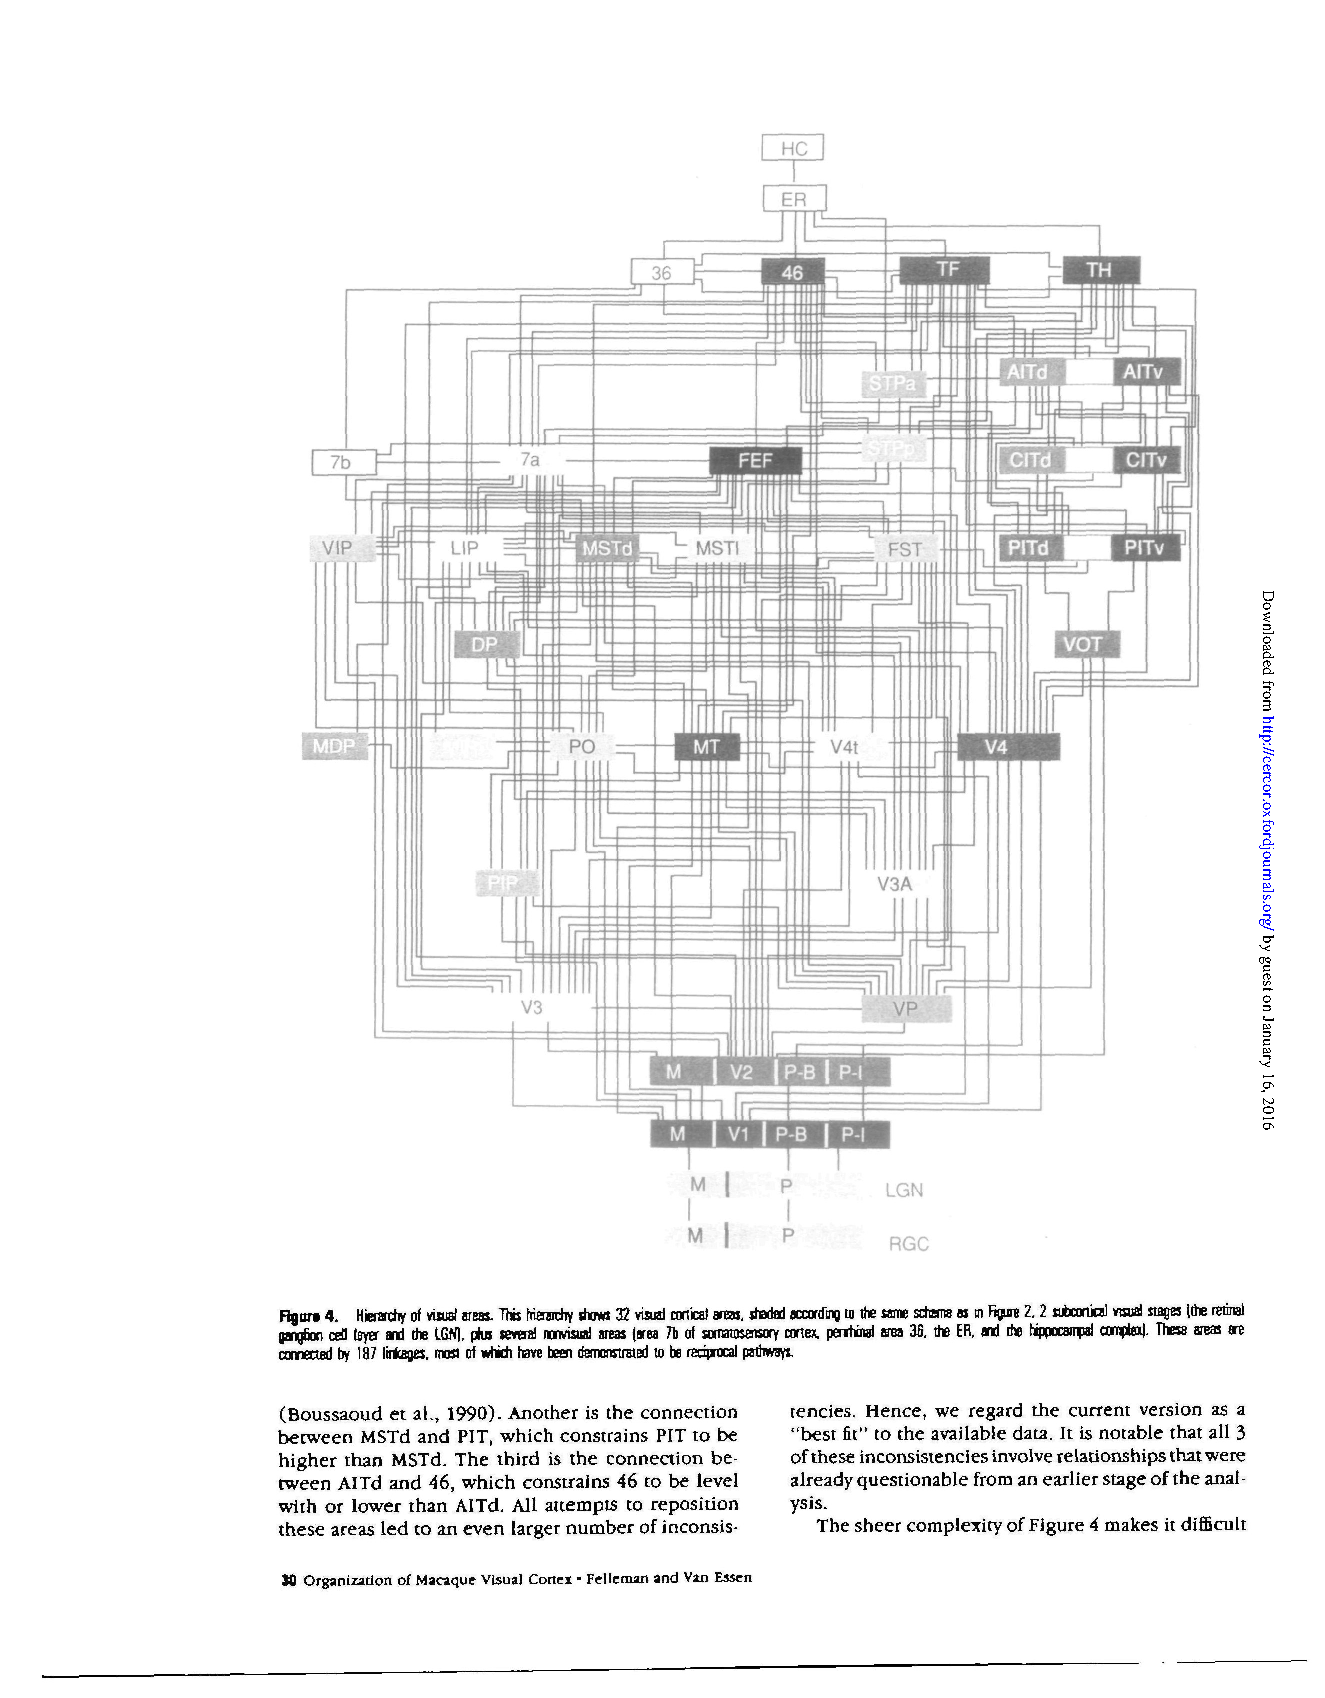
\includegraphics[width=\textwidth, trim=5cm 7cm 2cm 2cm, clip]{images/visual-cortex-map.pdf}
			\caption{Visual cortex map from retina (bottom) to hippocampus (top), most connection are reciprocal \citep{felleman1991distributed}}
			\label{cortex-map}
		\end{figure}
		
		Typically the visual cortex is separated in multiple major areas which are: the primary visual cortex V1 or the striate cortex and the extrastriate areas which are V2 to V5. The information processing is divided into two pathways: The dorsal visual pathway deals with calculating the location of objects meaning a 3D representation and is the connection of the visual cortex with the pariental lobe. The more important one is the ventral visual pathway that conducts the task of what the eyes see and leads to the temporal lobe.
		
		\begin{figure}[H]
			\centering
			\captionsetup{justification=centering,margin=2.3cm}
			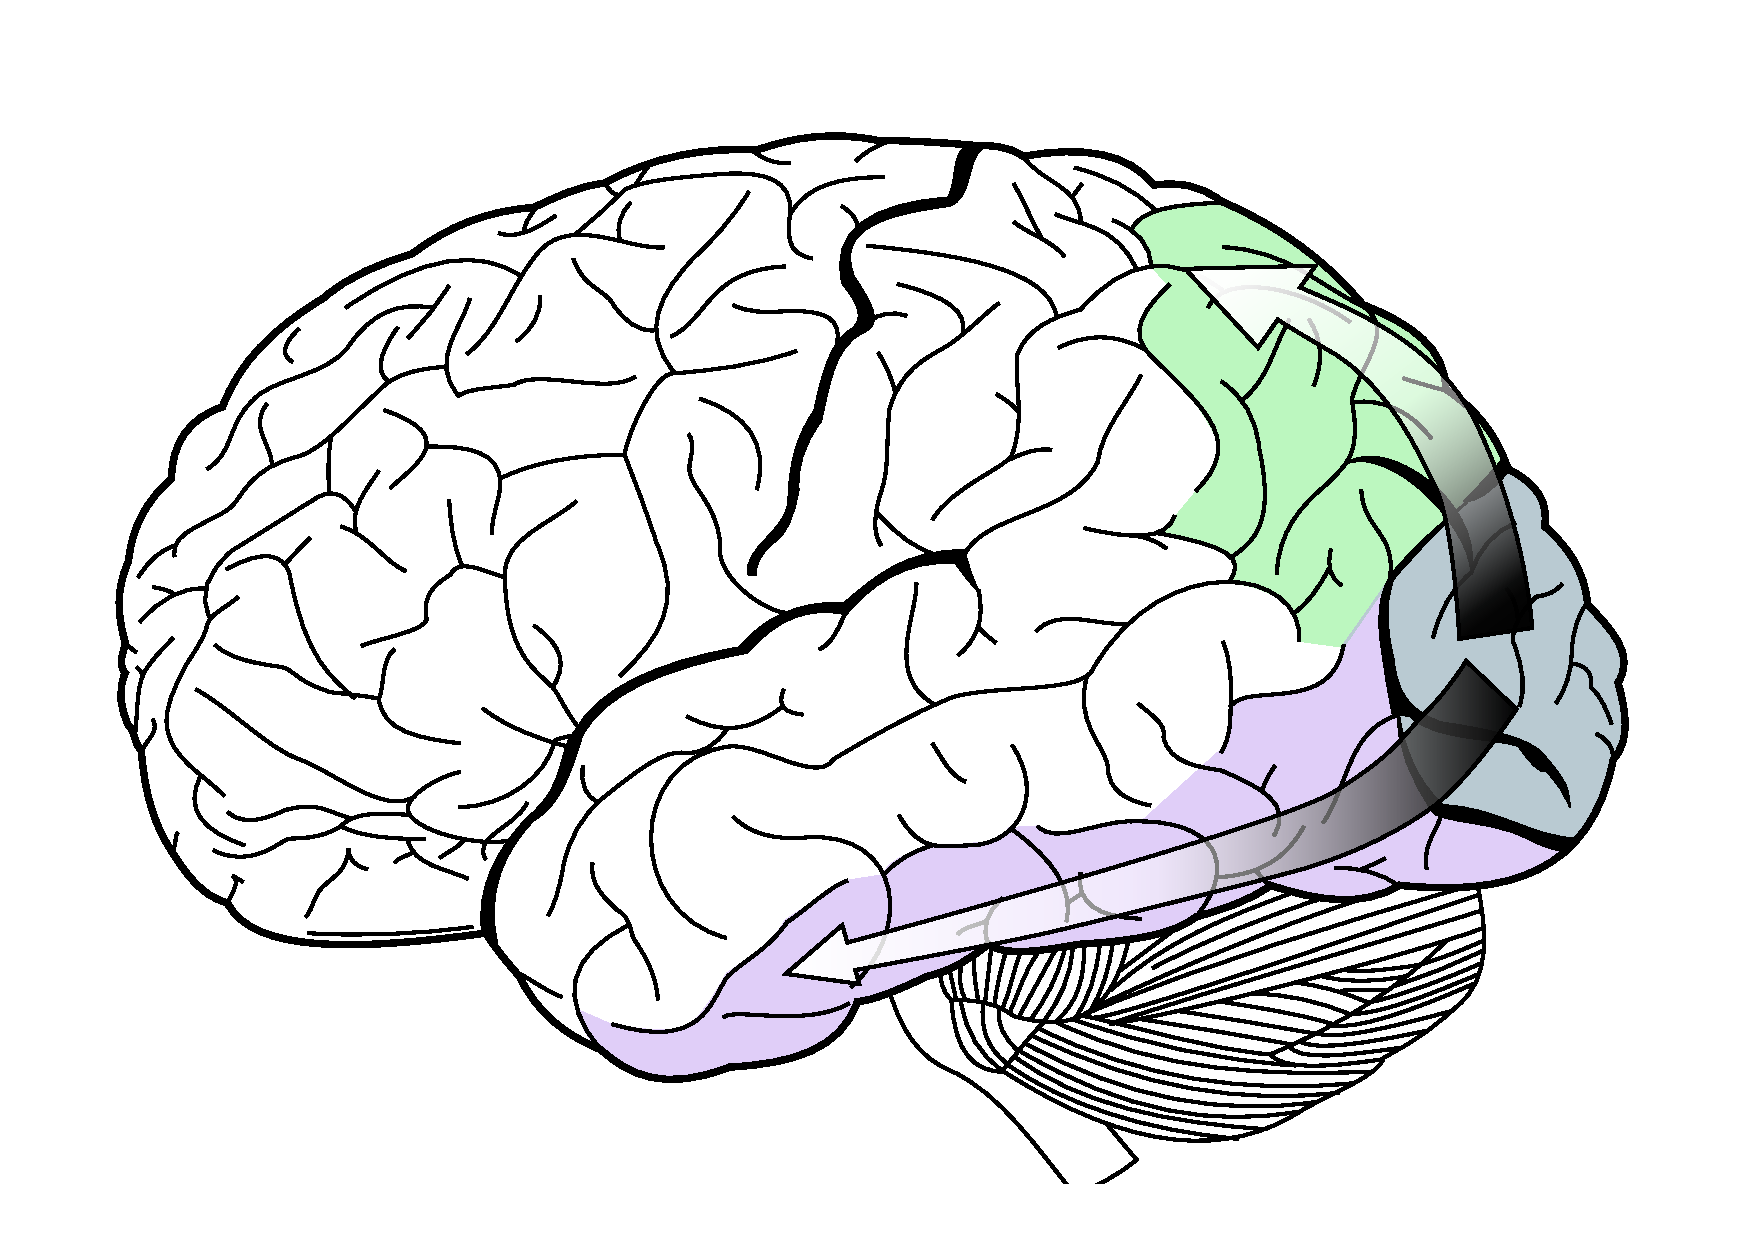
\includegraphics[width=0.7\textwidth]{images/visual-stream2.pdf}
			\caption{Ventral (purple) stream going to temporal lobe and dorsal (green) stream heading to parietal lobe [Source: scholarpedia.org]}
		\end{figure}
		
		In the first layer, the primary visual cortex, each neuron only responds to very little areas of the visual field. As the information over more and more neurons are combined in higher areas, each neuron represents the content of a larger receptive field. At the end invariance of position in the visual field is achieved, which means an object can be recognized no matter where on the input image it is. Simultaneously the selectivity is retained on higher levels with more complex patterns.
		
		As model to explain this was developed by \citeauthor{hubel1962receptive} with the use of simple and complex cells. It is described as part of the following chapter.
		
\chapter{Biologically Inspired Computational Models of the Visual System}

	Building a model for the visual system will be a compromise. Of course one can start to model every single neuron from the retina to the visual cortex, but this is very unpractical. So the typical step would be to abstract a certain part of the system to a functional description. There are basically two ways to do this: Abstraction top-down and bottom-up.
	
	Top-down means goal-driven, so you could build functional models that abstract viewing tasks, expectations or reasoning. Obviously this is very complicated, therefore bottom-up models, which are stimulus driven, are the way to go.
	
	To realize that kind of model, first of all the signal propagation in the visual system is summed up. Then with the research of \citep{hubel1962receptive} as basis the HMAX model will be explained.

%	\section{Types of Models}
%		
%		- start to abstract functional entities
%			- first model a neuron
%			- second model a bunch of neurons (functional areas)
%		
%		\subsection{Numerical Simulations}
%		
%			- simulating single neurons
%		
%			- very impractical because of high computational efforts, slow
%		
%		\subsection{Functional Models}
%
%			bottom-up vs top-down
%			
%			- stimulus-driven: characteristics like luminance, contrast, ...
%			
%			- top-down (goal driven): viewing task, expectations based on other stimuli or memory, temporal continuity, reasoning (visual attention)
	
		
	\section{Signal Propagation}
		
		The only connection of the retina is the optic nerve. It is about 1 million axons transmitting information in one direction, hence only feed-forward.
		
		Each additional layer of the visual path has back some sort of feedback. As mentioned in chapter 2, almost every connection in figure \ref{cortex-map} is bidirectional. This makes modeling extremely difficult. \citeauthor{thorpe1996speed} found out that even every cortex area of the visual system has some sort of higher function level feedback, in the first 150 milliseconds it is not active. Therefore for this short time one can assume a strict feed-forward network. Despite the fact many features are missing, most models limit themselves to feed-forward.
		
		What does the feedback provided and why is it important?
		%todo
		
	\section{Simple and Complex Cells}
		
		Nobel prize winners \citep{hubel1962receptive}
		
	
		\begin{figure}[H]
			\centering
			\captionsetup{justification=centering,margin=1cm}
			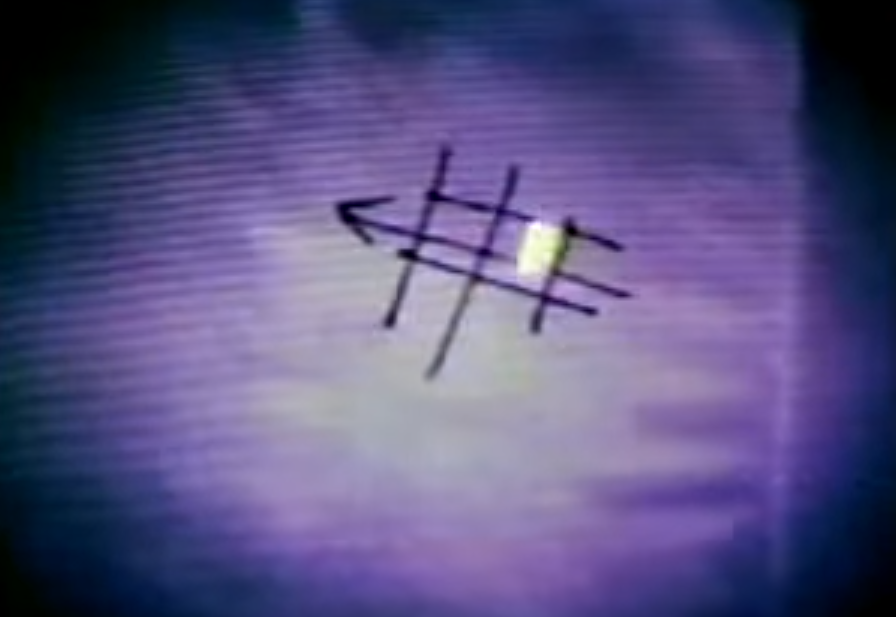
\includegraphics[width=0.5\textwidth]{images/hubel-experiment.png}
			\caption{Experiment performed by \citeauthor{hubel1962receptive}: Complex cell of a cat's visual cortex, the neuron fires only if a short bar is moved in the arrows direction [Source: youtube.com]}
		\end{figure}
		
	\section{HMAX models}
	
		\subsection{Only Feed-Forward model i.e. by Serre et al.}
		
			- simple and complex cells by hubel and wiesel
		
			- HMAX: Riesenhuber, Poggio extended this to object recognition
		
			- + feature learning at higher levels, switching to templates: Serre et al., Robust Object Recognition with Cortex-Like Mechanisms, 2007
			
		\subsection{Supervised Learning}
		
			- need for learning of localized objects by many pictures differing in
				- perspective
				- illuminance
				- ...
			
			- many examples per object needed
		
		\subsection{Biological plausibility}
		
			- no feedback
			
			- needs many examples for learning an object
				> Human can do this with only very few
			
			- clutter in scene causes big issues
			
			- Problems may be solved using feedback

			- +++ include hierarchy image

		\subsection{Comparison with State-of-the-Art Artificial Object Recognition}
		
			- common test framework: CaltecXYZ
		
			- regarding categorization, feature extraction (SIFT)
			
			\citep{serre2007robust}
 
\chapter{Application: Localization}

	- two approaches:
		- learning of every position individually: unpractical
		- learning the location of prominent objects and localize yourself using combinatiton of knowledge

	- so we go with the second approach

	- first, object recognition
	
	- second, location of the objects must be known
	
	- third, different information pieces must be put together for exact localization (particle filter) \citep{siagian2009biologically}


\chapter{Conclusion}

	still artificial RGB images are used, event based cameras are more biological accurate
	
